\chapter{Auswertung}\label{Chap:Eval}
Im folgenden soll betrachtet werden, wie gut der beschriebene Detektor 
in der Lage ist, Situationen wie in Kap. \ref{chap:introduction} 
beschrieben zu erkennen. Dabei werden sowohl künstlich konstruierte 
Situationen, als auch tatsächliche Programme betrachtet. Für die Betrachtung 
tatsächlicher Programme werden Programme aus GoBench bzw. Goker~\cite{gobench}
verwendet. Dabei handelt es sich um eine Sammlung von Programmteilen mit 
Concurrency-Bugs aus 9 
großen open-source Anwendungen wie z.B. Kubernetes und Moby. 
Beschreibungen der Probleme, sowie die Ergebnisse des Detektors befinden in 
Anhang~\ref{Appendix-1}.\\
Anschließend werden die Leistungen des Detektors mit denen von GFuzz verglichen.
\todo{wahrscheinlich nur channel}

\section{Standardprogramme}
Für die Analyse wurden insgesammt 35 Standartprobleme betrachtet. 
Dabei wurde überprüft, ob der Detektor in der Lage ist, das in dem 
Programm erhaltene Problem richtig zu erkennen, bzw.~zu erkenne wenn 
die vorliegende Situation nicht zu einem Problem führen kann. Eine 
tabellarische Beschreibung der betrachteten Situationen, sowie der Ergebnisse 
des Detektors ist in Tab.~\ref{App-Stand} in Anhang~\ref{Appendix-1} aufgeführt.
Abb.~\ref{Chap:Eval-Sec:Stand-Fig:Total} - \ref{Chap:Eval-Sec:Stand-Fig:Mix}
zeigen die Ergebnisse der Auswertung.\\\\
Von den 43 Programmen konnten 38 korrekt kategorisiert werden. Dabei 
bestehen 18 Probleme aus Problemen mit Mutexen (17 korrekt erkannt),
18 aus Problemen mit Channel (16 korrekt erkannt) und 7 mit einem 
Mix aus Mutexen und Channel (5 korrekt erkannt).



Zuerst sollen Standardprogramme betrachtet werden, die durch Mutexe erzeugte 
Bug enthalten, sowie Probleme mit Mutexen, in denen keine Probleme enthalten 
sind, welche durch eine Detektor aber fälschlicherweise für solche gehalten werden 
könnten. Eine Liste der betrachteten Probleme befinden sich in 
Tab.~\ref{App-Stand}. Von den 22 betrachteten Problemen war es des 
Detektor in 19 Fällen möglich, die Situation richtig zu erkennen. Lediglich 
in einer Situation war es dem Detektor nicht möglich, einen potenziellen 
Deadlock zu erkennen. Dabei handelt es sich um eine Situation, bei der 
ein potenzielles doppeltes Locking durch verschachtelte Routinen verschleiert 
wird. Da die innere Routine als eigenständige Routine angesehen wird, 
werden Abhängigkeiten der Lock-Operationen nicht in den Lock-Bäumen abgebildet 
und könne daher auch nicht erkannt werden. \\



\begin{minipage}{0.45\textwidth}
  \centering  
  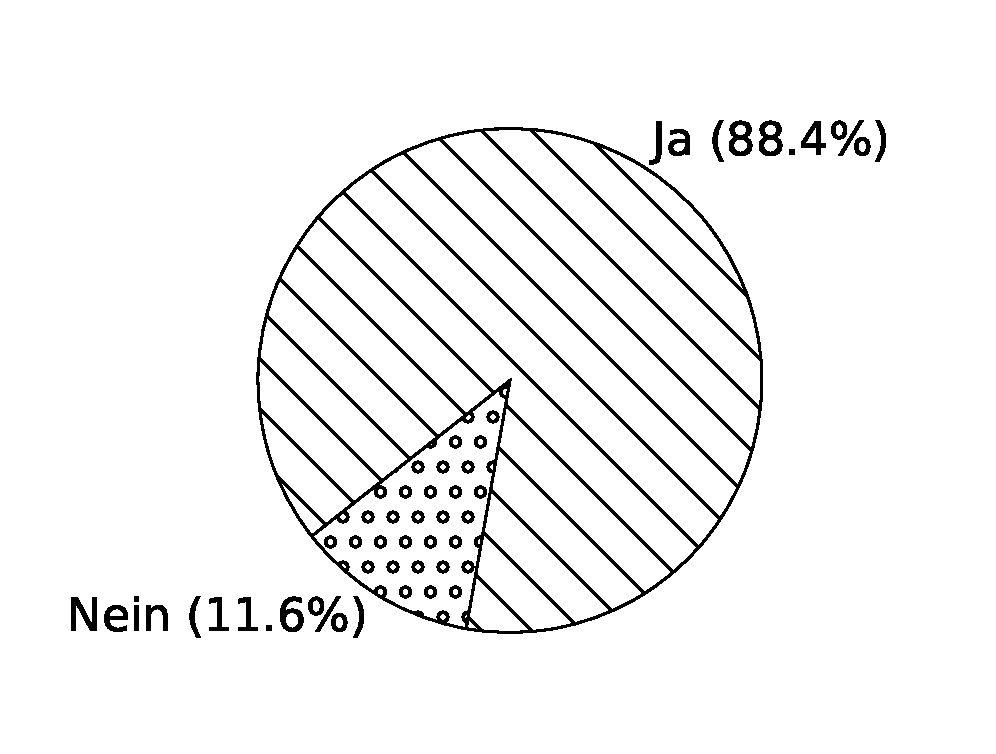
\includegraphics[width=0.8\textwidth]{img/pi_standard_total.eps}
  \captionof{figure}{Verteilung der Ergebnisse für Standardprogramme}
  \label{Chap:Eval-Sec:Stand-Fig:Total}
\end{minipage}
\hfill
\begin{minipage}{0.45\textwidth}
  \centering
  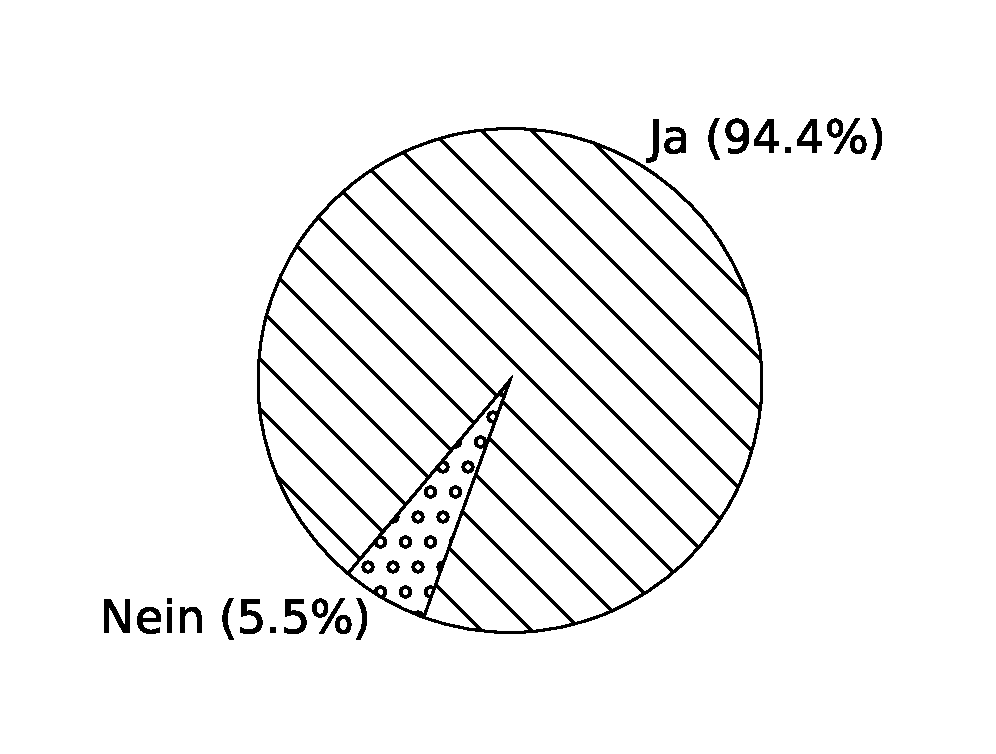
\includegraphics[width=0.8\textwidth]{img/pi_standard_mutex.eps}
  \captionof{figure}{Verteilung der Ergebnisse für Standardprogramme mit Mutexen}
  \label{Chap:Eval-Sec:Stand-Fig:Mutex}
\end{minipage}
\begin{minipage}{0.45\textwidth}
  \centering  
  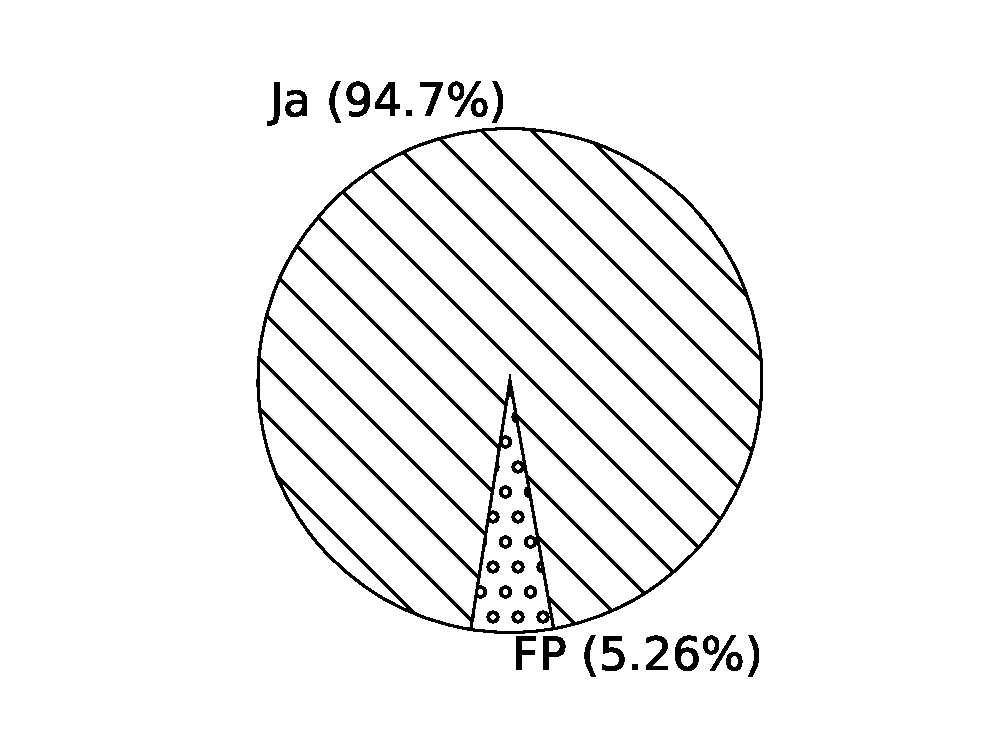
\includegraphics[width=0.8\textwidth]{img/pi_standard_channel.eps}
  \captionof{figure}{Verteilung der Ergebnisse für Standardprogramme mit Channel}
  \label{Chap:Eval-Sec:Stand-Fig:Channel}
\end{minipage}
\hfill
\begin{minipage}{0.45\textwidth}
  \centering
  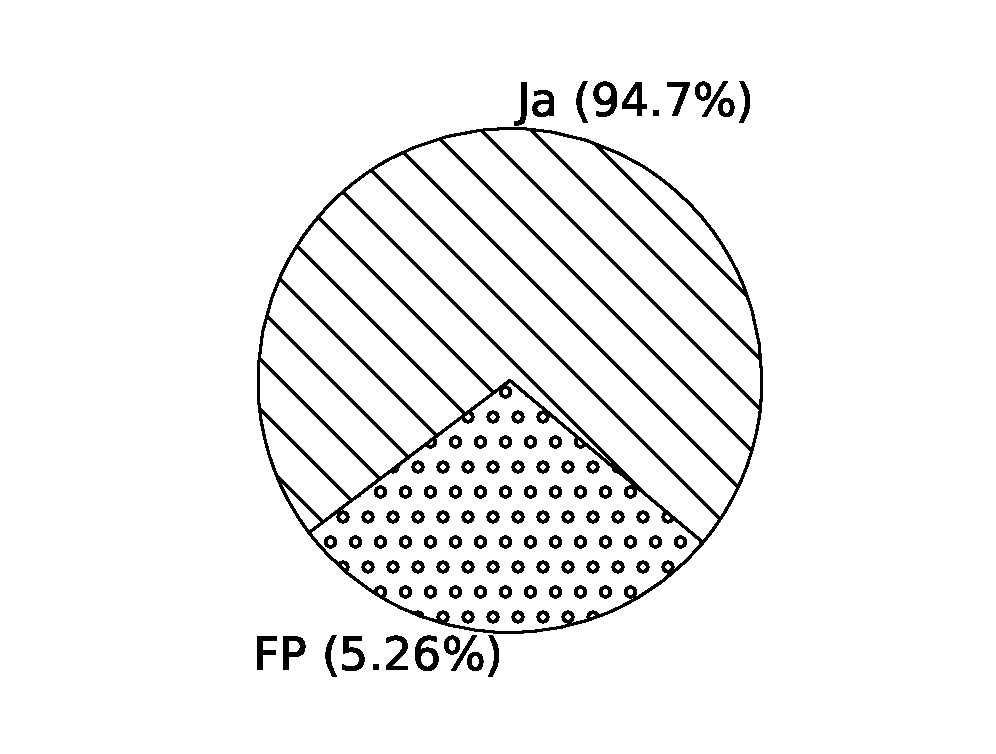
\includegraphics[width=0.8\textwidth]{img/pi_standard_mix.eps}
  \captionof{figure}{Verteilung der Ergebnisse für Standardprogramme mit Mutexen und Channel}
  \label{Chap:Eval-Sec:Stand-Fig:Mix}
\end{minipage}
\todo{cont. Beschreibung}

\section{Goker}
Für die Analyse wurden insgesamt 35 Programme betrachtet. Die betrachteten 
Programme und deren Ergebnisse befinden sich in Tab.~\ref{App-Goker} 
in Anhang~\ref{Appendix-1}. Von den Programmen betrafen 15 die 
Verwendung von Resource wie Mutexen (14 korrekt erkannt), 11 die 
Verwendung von Kommunikationen und 9 eine Kombination aus Mutexen und 
Channel (7 korrekt erkannt). \\

\begin{minipage}{0.45\textwidth}
  \centering  
  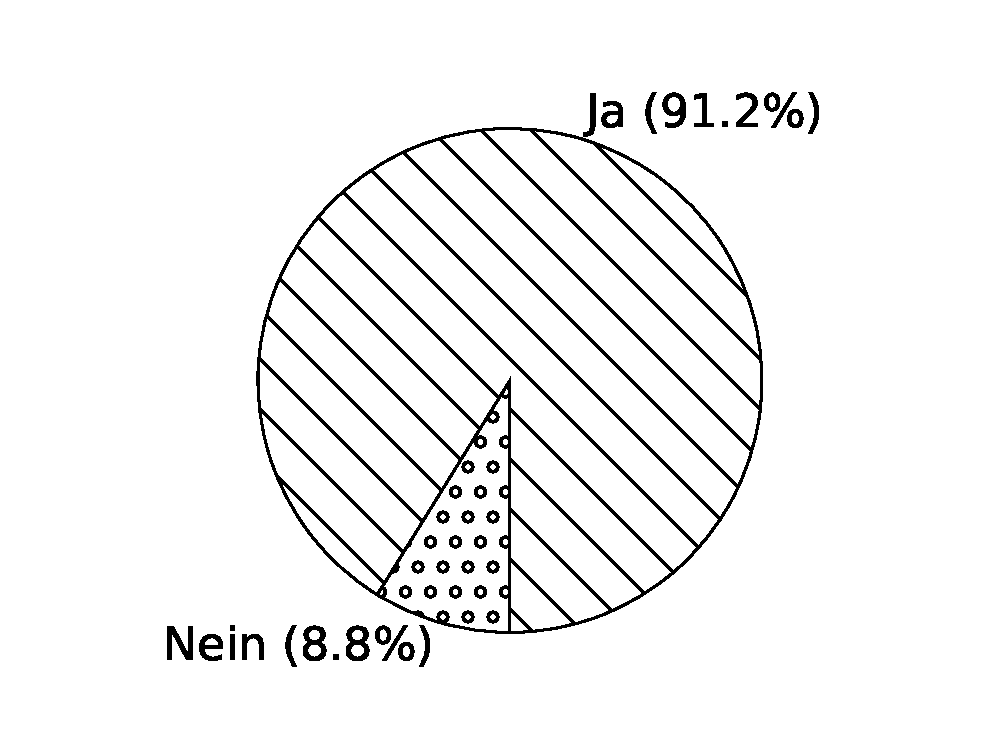
\includegraphics[width=0.8\textwidth]{img/pi_goker_total.eps}
  \captionof{figure}{Verteilung der Ergebnisse für Programme aus GoKer}
  \label{Chap:Eval-Sec:Goker-Fig:Total}
\end{minipage}
\hfill
\begin{minipage}{0.45\textwidth}
  \centering
  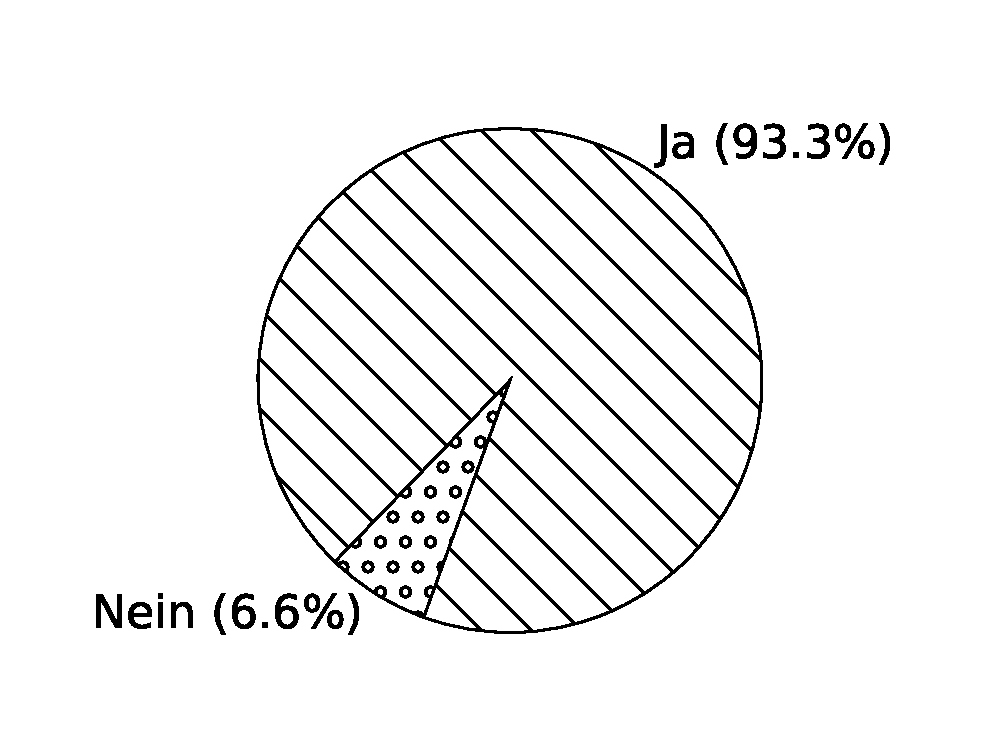
\includegraphics[width=0.8\textwidth]{img/pi_goker_mutex.eps}
  \captionof{figure}{Verteilung der Ergebnisse für Programme aus GoKer mit Mutexen}
  \label{Chap:Eval-Sec:Goker-Fig:Mutex}
\end{minipage}
\begin{minipage}{0.45\textwidth}
  \centering  
  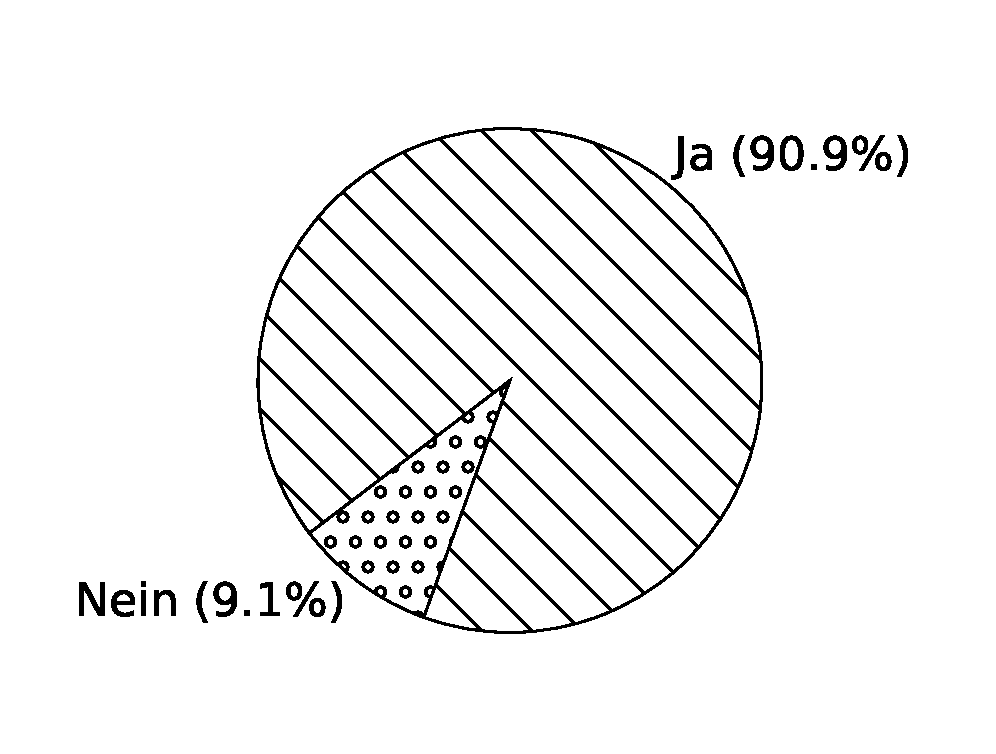
\includegraphics[width=0.8\textwidth]{img/pi_goker_channel.eps}
  \captionof{figure}{Verteilung der Ergebnisse für Programme aus GoKer mit Channel}
  \label{Chap:Eval-Sec:Goker-Fig:Channel}
\end{minipage}
\hfill
\begin{minipage}{0.45\textwidth}
  \centering
  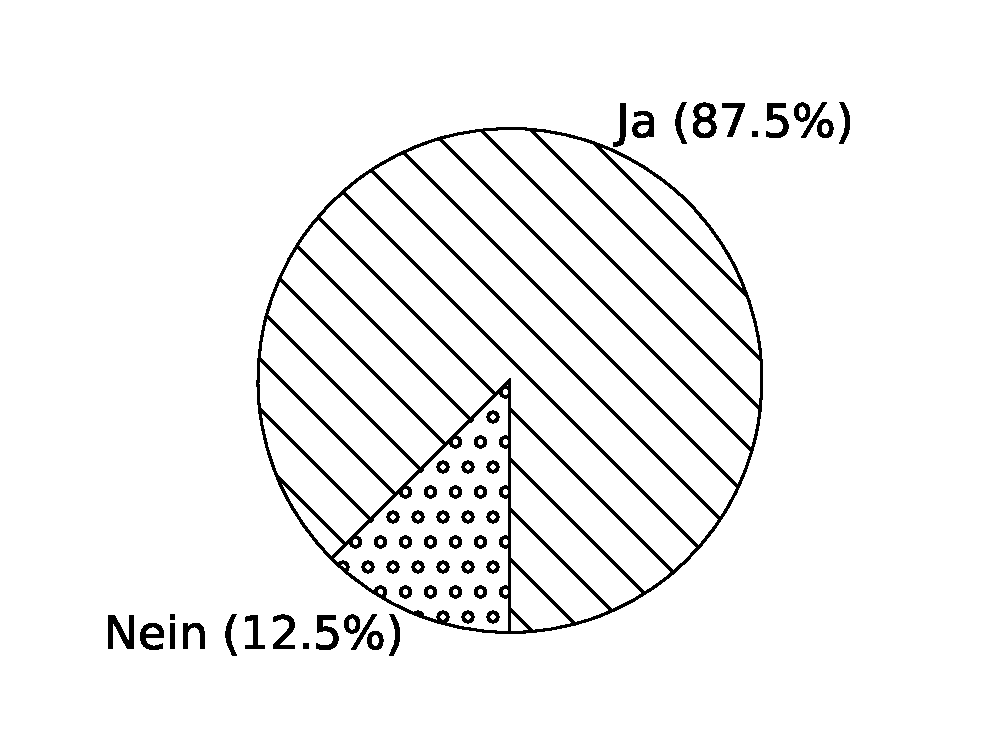
\includegraphics[width=0.8\textwidth]{img/pi_goker_mix.eps}
  \captionof{figure}{Verteilung der Ergebnisse für Programme aus GoKer mit Mutexen und Channel}
  \label{Chap:Eval-Sec:Goker-Fig:Mix}
\end{minipage}
\todo{Beschreibung der Messwerte}

\section{Vergleich mit GFuzz}
\todo{Vergleich mit GFuzz}








\todo{Funktioniert nicht, wenn externe Funktionen auf Chan or Mut verwendet werden}